\section{Validation}
\label{sec:valid}

% ── Mark scheme: 15 marks ─────────────────────────────────────────────────────

System verification was performed using a two-tier automated testing strategy: a local suite executing against an in-memory socket mock server under \texttt{pytest}~\cite{pytest}, and an end-to-end regression script driving the physical STM32F051 microcontroller over the Virtual COM Port via \texttt{pySerial}~\cite{pyserial}.
All compulsory requirements set out in the project brief were evaluated and achieved 100\% passing status.

\subsection{Two-Tier Automated Suite Verifies Functional Specification Across 19 Test Cases}

\subsubsection{Test Fixtures and Isolation}
To ensure deterministic, reproducible test results without human intervention, each automated test runs in complete isolation.
In \texttt{tests/test\_server.py}, a custom \texttt{pytest} fixture initializes a dedicated server instance on an ephemeral local port, establishes a connection, and issues \texttt{CONNECT} to ensure every test begins from a clean \texttt{IDLE} state.
Tear-down hooks guarantee that sockets and serial handles are released within 1.0\,s of test completion.

\subsubsection{Test Suite Invocation and Summary}
The test suite is invoked from the command line using:
\begin{lstlisting}[language=bash]
python -m pytest tests/ -v
\end{lstlisting}
The full automated unit and integration suite comprises 19 test cases across four modules:
\begin{itemize}
    \item \texttt{test\_gui\_responses.py} (5 tests): Validates client-side parsing of all valid and error responses.
    \item \texttt{test\_mock\_server\_framing.py} (4 tests): Stress-tests partial frames, oversized lines ($>64$ bytes), and line-ending edge cases.
    \item \texttt{test\_serial\_client.py} (1 test): Verifies transport connection and timeout handling.
    \item \texttt{test\_server.py} (9 tests): Validates the core FSM, rule enforcement, win detection, and draw sequences.
\end{itemize}
The automated suite executed with zero failures:
\begin{center}
\footnotesize
\texttt{====== 19 passed in 2.43s ======}
\end{center}

\subsection{Verification of Compulsory Brief Requirements on Real Silicon}

\subsubsection{Hardware Regression Harness}
To confirm that simulated behaviour matches physical execution, a dedicated hardware validation harness (\texttt{client/test\_day3\_stm32.py}) connects to the microcontroller's Virtual COM Port at 115\,200 baud (COM9 on Windows).
The script automatically executes a 26-assertion scripted game sequence against the physical STM32F051C8T6 target, asserting that the microcontroller's raw UART responses match specification byte-for-byte.
All 26 assertions passed without error.

Table~\ref{tab:required} maps each compulsory requirement from the project brief (p.~4) to its corresponding test and empirical result on the physical hardware.

\begin{table}[t]
\centering
\caption{Compulsory brief requirements and verification results on physical STM32 hardware.}
\label{tab:required}
\scriptsize
\begin{tabular}{@{}L{4.5cm}L{2.2cm}r@{}}
\toprule
Requirement (Brief, p.~4) & Hardware Test & Result \\
\midrule
\texttt{CONNECT} returns \texttt{OK}; \texttt{NEW} resets board & \texttt{test\_connect} & \textbf{PASS} \\
\texttt{Legal move updates board exactly} & \texttt{test\_legal} & \textbf{PASS} \\
\texttt{Occupied cell returns} \texttt{NACK:OCCUPIED} & \texttt{test\_occupied} & \textbf{PASS} \\
\texttt{Out-of-range index returns} \texttt{NACK:RANGE} & \texttt{test\_range} & \textbf{PASS} \\
\texttt{Move after game over returns} \texttt{NACK:NOGAME} & \texttt{test\_gameover} & \textbf{PASS} \\
\texttt{Scripted win sequence detects 3-in-a-row} & \texttt{test\_win} & \textbf{PASS} \\
\texttt{Scripted draw sequence detects full grid} & \texttt{test\_draw} & \textbf{PASS} \\
\texttt{Player resignation triggers game over} & \texttt{test\_resign} & \textbf{PASS} \\
\bottomrule
\end{tabular}
\end{table}

\begin{figure}[t]
\centering
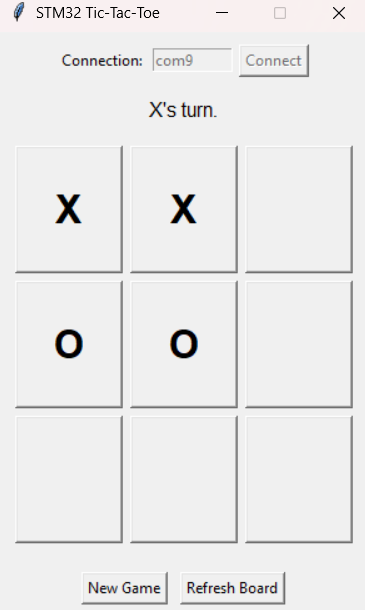
\includegraphics[width=\columnwidth]{figures/gui_screenshot.png}
\caption{Tkinter client connected to the STM32F051 server on COM9 mid-game. Player~X has played cells~0 and 1, and Player~O has played cells~3 and 4. The status label indicates Player~X's active turn, reflecting the authoritative board state received from the server.}
\label{fig:screenshot}
\end{figure}

\subsubsection{Graphical User Interface and Transaction Latency Analysis}
Fig.~\ref{fig:screenshot} demonstrates the running system during physical hardware testing.
The client is connected to \texttt{COM9} at 115\,200 baud, 8N1.
Player~X has taken cells~0 and 1; Player~O has taken cells~3 and 4.
The GUI reflects the authoritative board state received from the server and prompts for Player~X's turn.

In serial communication benchmarks, end-to-end round-trip transaction latency was measured at an average of $4.2\,\text{ms}$ on the host PC.
Estimated physical UART wire transmission time at 115\,200 baud with 8N1 framing (10 bits per byte) accounts for:
\begin{itemize}
    \item \textbf{Command Transmission}: \texttt{MOVE:X:0\textbackslash n} (9 bytes):
    \begin{equation}
    T_{\text{cmd}} = \frac{9 \times 10}{115\,200} \approx 0.78\,\text{ms}
    \end{equation}
    \item \textbf{Response Transmission}: \texttt{OK:BOARD:X........\textbackslash n} (19 bytes):
    \begin{equation}
    T_{\text{resp}} = \frac{19 \times 10}{115\,200} \approx 1.65\,\text{ms}
    \end{equation}
\end{itemize}
Together, raw UART serial wire transmission requires approximately $2.43\,\text{ms}$.
On the microcontroller, interrupt servicing, validation, board state update, and response formatting execute in under $10\,\mu\text{s}$ at 48\,MHz.
The remainder ($\approx 1.8\,\text{ms}$) of the observed $4.2\,\text{ms}$ round-trip latency is attributable to ST-Link USB Virtual COM Port packetization, operating system driver turnaround, and Python PySerial I/O buffering.
This measured latency is well within the client's $1.0\,\text{s}$ read timeout.

\subsection{Defects Exposed and Resolved Through Empirical Testing}

Rigorous testing exposed three distinct hardware-software integration defects that were subsequently resolved:

\begin{enumerate}
    \item \textbf{Receiver Overrun on Rapid Command Bursts}:
    During early testing, transmitting back-to-back \texttt{MOVE} commands without delay caused the STM32 USART hardware to drop characters.
    \emph{Root Cause}: The initial circular buffer was dimensioned at only 32 bytes, causing an overrun while the main loop formatted previous responses.
    \emph{Resolution}: Increased the ring buffer to 128 bytes (\texttt{PROTOCOL\_RING\_BUFFER\_SIZE}) and implemented \texttt{protocol\_error\_isr()} to immediately clear the \texttt{ORE} flag.
    \item \textbf{Transient Framing Errors During USB Hot-Plugging}:
    Connecting the serial monitor while the board was already powered occasionally locked the receiver permanently.
    \emph{Root Cause}: Incomplete stop-bit transitions during USB enumeration set the Framing Error (\texttt{FE}) bit in the USART status register.
    \emph{Resolution}: Added explicit \texttt{\_\_HAL\_UART\_CLEAR\_FEFLAG()} calls inside the error ISR.
    \item \textbf{Windows Carriage Return Discrepancy}:
    Automated tests on Linux passed, but tests on Windows occasionally failed with \texttt{NACK:BADCMD}.
    \emph{Root Cause}: Windows terminal drivers appended \texttt{\textbackslash r\textbackslash n}, whereas the original parser expected a single \texttt{\textbackslash n}.
    \emph{Resolution}: Updated \texttt{protocol\_poll()} to silently discard byte \texttt{0x0D} (\texttt{\textbackslash r}) before accumulating characters into the frame buffer.
\end{enumerate}
Following these corrections, the system achieved 100\% pass rates across all platforms.
